%%%%%%%%%%%%%%%%%%%%%%%%%%%%%%%%%%%%%%%%%%%%%%%%%%%%%%%%%%%%%%%%%%%%
%% I, the copyright holder of this work, release this work into the
%% public domain. This applies worldwide. In some countries this may
%% not be legally possible; if so: I grant anyone the right to use
%% this work for any purpose, without any conditions, unless such
%% conditions are required by law.
%%%%%%%%%%%%%%%%%%%%%%%%%%%%%%%%%%%%%%%%%%%%%%%%%%%%%%%%%%%%%%%%%%%%

\documentclass{beamer}
\usetheme[faculty=phil, logo = minerva.png]{fibeamer}
\usepackage[utf8]{inputenc}
\usepackage[
  main=english, %% By using `czech` or `slovak` as the main locale
                %% instead of `english`, you can typeset the
                %% presentation in either Czech or Slovak,
                %% respectively.
  czech, slovak %% The additional keys allow foreign texts to be
]{babel}        %% typeset as follows:
%%
%%   \begin{otherlanguage}{czech}   ... \end{otherlanguage}
%%   \begin{otherlanguage}{slovak}  ... \end{otherlanguage}
%%
%% These macros specify information about the presentation
\title{Um estudo sobre metódos simpléticos} %% that will be typeset on the
\subtitle{Solução Númerica do problema dos n-corpos} %% title page.
\author{Gil Sales M. Neto \\ {\tiny Trabalho Final de ANEDO}}
%% These additional packages are used within the document:
\usepackage{ragged2e}  % `\justifying` text
\usepackage{booktabs}  % Tables
\usepackage{tabularx}
\usepackage{tikz}      % Diagrams
\usetikzlibrary{calc, shapes, backgrounds}
\usepackage{amsmath, amssymb}
\usepackage{url}       % `\url`s
\usepackage{listings}  % Code listings
\frenchspacing
\begin{document}
  \frame{\maketitle}


    \section{Light Frames}
    \subsection{Blind Text}
    \begin{frame}{O Problema dos N-Corpos}
      \framesubtitle{}%
      \begin{itemize}
      \item O problema dos dois, três ou n-corpos é um problema de mecânica clássica que modela o movimento de \(n\) partículas que interagem entre com uma força gravitacional.
      \item O movimento é calculado utilizando as Leis de Movimento de Newton, e a Lei da Gravitação Universal de Newton.
      \item Há atualmente aproximadamente 1800 satélites artificais orbitando a Terra.
    \end{itemize}
    \end{frame}

    \begin{frame}{One Equation to rule them all}
      \framesubtitle{One Equation to \alert{find} them all}%
      A segunda lei de Newton
      \[F = ma\]
      A Lei da Gravitação Universal
      \[F = G \cdot \frac{m_1 m_2}{r ^2}\]
      The One Differential equation
      \[
        m_1a = G \cdot \frac{m_1 m_2}{r ^2} \implies \ddot{r} = G \cdot \frac{m_2}{\lVert r \rVert ^2}
      \]
    \end{frame}

    \begin{frame}{Redução de ordem da EDO e sistema de Equações}
      \framesubtitle{}%
      A equação diferencial
      \[
        \ddot{r_i} = G \cdot \sum_{j = 0}^{n}\frac{m_j}{\lVert r_{i,j} \rVert ^2}
      \]
      Reduzindo a um sistema de equações
      \[
      \begin{cases}
        \frac{\mathrm{d}r_i}{\mathrm{d}t} = v_i \\
        \frac{\mathrm{d}v_i}{\mathrm{d}t} = G \cdot \displaystyle \sum_{j = 0}^{n}\frac{m_j}{\lVert r_{i,j} \rVert ^2}
      \end{cases}
      \]
      E resolvendo esse sistema de equações podemos determinar a posição do corpo \(i\)
    \end{frame}

    \begin{frame}{As leis físicas que regem o movimento dos planetas}
      \framesubtitle{As 3 leis de Kepler}%
          \begin{enumerate}
            \item Planetas se movem ao redor do Sol em órbitas Elipticas, com o Sol em um dos focos
            \item Um planeta varre a mesma área em um mesmo período de tempo
            \item Os quadrados dos períodos de revolução dos planetas são diretamente proporcionais aos cubos dos raios médios de suas órbitas
          \end{enumerate}
    \end{frame}
    \begin{frame}{As leis físicas que regem o movimento dos planetas}
      \framesubtitle{Hamiltoniano e Momento Angular}%
          \begin{itemize}
            \item \(U = G \displaystyle \sum_{i,j}^n \frac{m_i m_j}{\lVert q_i - q_j \rVert}\),\, \, \,  \, \, \, \, Self Potential Energy
            \item \( p_i = m_i \dot{q_i} \) \, \, \, \, \, \, \, \, \, \, \, \, \, \, \, \, \, \, \, \, \,   Momento Linear
            \item \(H = \displaystyle \sum_{i = 1}^{n} \frac{\lVert p_i \rVert ^2}{2m_i} - U\), \, \, \, \, \, \, \, \, \,  Hamiltoniano
            \item \(L = q \times p\), \, \, \, \, \, \, \, \, \, \, \, \, \, \, \, \,  Momento Angular
            \item \( \lVert L \rVert &= \sqrt{\rVert q \lVert^2 \rVert p \lVert^2(sin(\theta))^2} = \sqrt{\rVert q \lVert^2 \rVert p \lVert^2 - \langle q, p \rangle ^2}\)
          \end{itemize}
    \end{frame}


    \begin{frame}{Discretização da EDO}
      \framesubtitle{O Metódo de Euler}%
      Podemos discretizar a nossa equação diferencial com base no metódo de Euler, que é um metódo de passo explicito.\\
      A discretização é feita com a expansão em Série de Taylor das equações diferenciais
      \[
      \begin{cases}
        r_{t+1} = r_{t} + \Delta t \cdot v_t\\
        v_{t+1} = v_{t} + \Delta t \cdot a_t
      \end{cases}
      \]
    \end{frame}

    \begin{frame}{Definindo valores iniciais}
      \[
      \begin{cases}
        r_x(0) = \text{Afélio}\\
        r_y(0) = 0\\
        v_x(0) = 0\\
        v_y(0) =  \text{Velocidade orbital média}
      \end{cases}
      \]
      \url{https://nssdc.gsfc.nasa.gov/planetary/factsheet/}
    \end{frame}

    \begin{frame}
      \begin{figure}[h]
        \vspace{-0.5cm}
        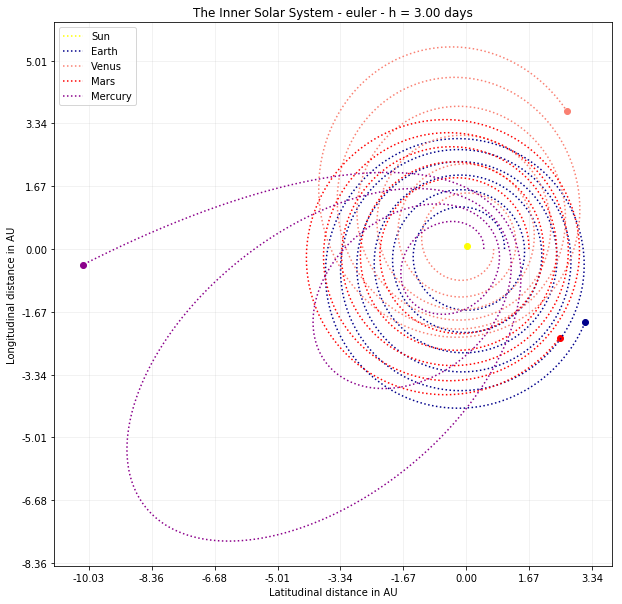
\includegraphics[width=110mm, height = 90mm]{resources/earth_wrong.png}
      \end{figure}
    \end{frame}

    \begin{frame}{O que deu errado?}
      \framesubtitle{Integradores Simpléticos}%
      O metódo de Euler explicito conserva apenas aproximadamente a energia do sistema.\\
      Metódos simpléticos conservam exatamente uma quantia que aproximadamente é a Energia do sistema.\\
      \caption{Integradores Simpléticos}
      \begin{itemize}
        \item Euler-Cromer
        \item Velocity-Verlet
        \item 7 Step Verlet (Leapfrog)
      \end{itemize}
    \end{frame}
    \begin{frame}{Integradores Simpléticos}
      \framesubtitle{Vantagens}%
      \begin{itemize}
        \item Podem 'voltar no tempo'
        \item Conservam momento Angular
        \item Simpléticos (presevam área)
      \end{itemize}
    \end{frame}

    \begin{frame}{Euler-Cromer}
      \framesubtitle{Verlet-Stormer (Euler semi-implicito 1ª ordem)}%
      \[
      \begin{cases}
        v_{t+1} = v_{t} + \Delta t \cdot a_t\\
        r_{t+1} = r_{t} + \Delta t \cdot v_{t+1}
      \end{cases}
      \]
    \end{frame}

    \begin{frame}
      \begin{figure}[h]
        \vspace{-0.5cm}
        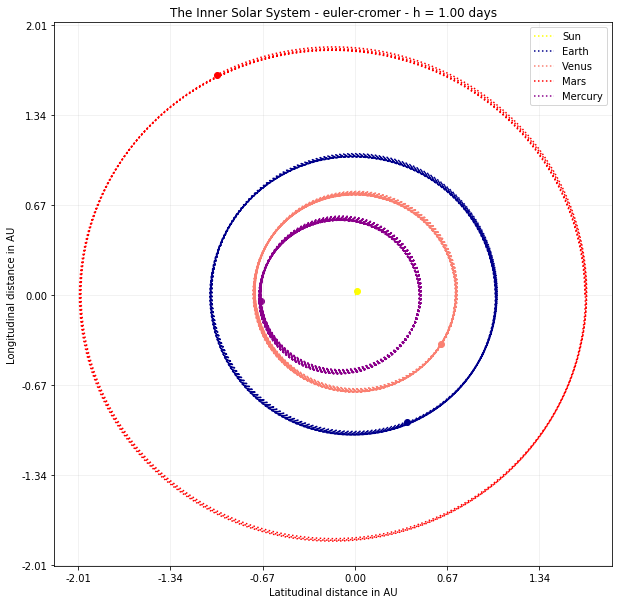
\includegraphics[width=110mm, height = 90mm]{resources/euler_cromer.png}
      \end{figure}
    \end{frame}

    \begin{frame}{Integrador de Verlet de 3 passos}
      \framesubtitle{Velocity Verlet (2ª ordem)}%

      \[
      \begin{cases}
        v_{t_\frac{1}{2}} = v_t + \frac{1}{2} \Delta t \cdot a_t  \\
        r_{t+1} = r_t + \Delta t \cdot v_{t\frac{1}{2}} \\
        v_{t+1} = v_{t\frac{1}{2}} + \frac{1}{2}\Delta t\cdot A(r_{t+1})
      \end{cases}
      \]
    \end{frame}

    \begin{frame}
      \begin{figure}[h]
        \vspace{-0.5cm}
        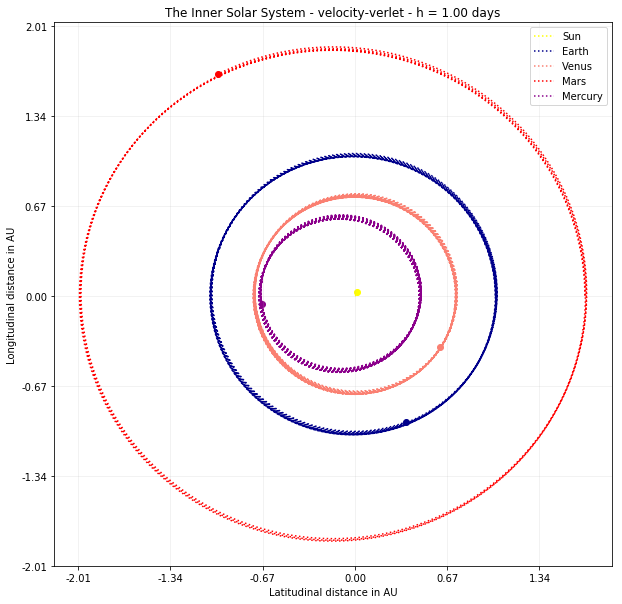
\includegraphics[width=110mm, height = 90mm]{resources/verlet.png}
      \end{figure}
    \end{frame}

    \begin{frame}{Integrador de Verlet de 7 passos}
      \framesubtitle{Leapfrog}%
      \begin{figure}[h]
        \vspace{-0.5cm}
        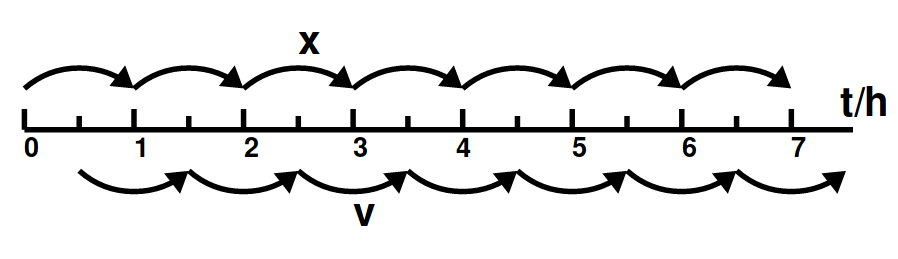
\includegraphics[width=50mm, height = 30mm]{resources/leap_scheme.png}
      \end{figure}
    \end{frame}

    \begin{frame}{Integrador de Verlet de 7 passos}
      \framesubtitle{Leapfrog}%
      \begin{columns}[onlytextwidth]
        \column{.5\textwidth}
      \[
      \begin{cases}
        w &= \sqrt[3]{2}\\
        f &= 2 - w\\
        leap_1 = leap_7 &= \frac{h}{2f}\\
        leap_2 = leap_6 &= \frac{h}{f}\\
        leap_3 = leap_5 &= (1-w) \frac{h}{2f}\\
        leap_4 &= -h \frac{w}{f}
      \end{cases}
      \]
      \column{.5\textwidth}
      \[
      \begin{cases}
      x_{1} &= x_t + leap_1 \cdot v_t\\
      v_{2} &= v_t + leap_2 \cdot A(x_{1})\\
      x_{3} &= x_{1} + leap_3 \cdot v_{2}\\
      v_{4} &= v_{2} + leap_4 \cdot A(x_{3})\\
      x_{5} &= x_{3} + leap_5 \cdot v_{4}\\
      v_{t+1} &= v_{4} + leap_6 \cdot A(x_{5})\\
      x_{t+1} &= x_{5} + leap_7 \cdot v_{t+1}
    \end{cases}
    \]
    \end{columns}
    \end{frame}

    \begin{frame}
      \begin{figure}[h]
        \vspace{-0.5cm}
        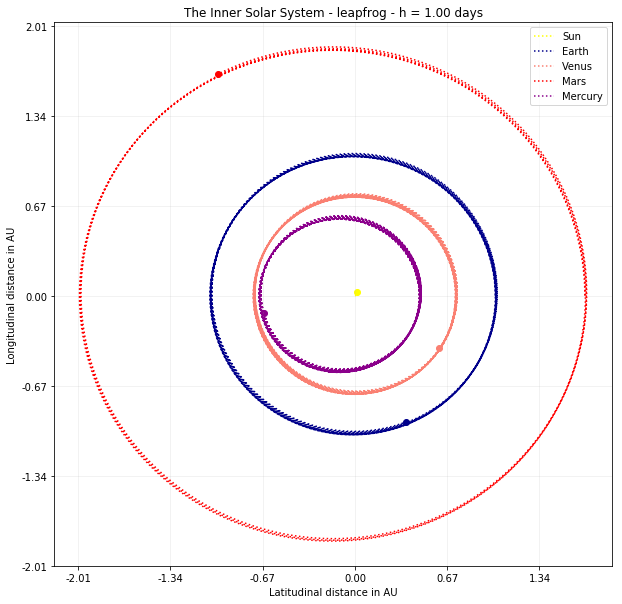
\includegraphics[width=110mm, height = 90mm]{resources/leap1.png}
      \end{figure}
    \end{frame}

    \begin{frame}{Conservação do Hamiltoniano}

      \begin{figure}[h]
        \vspace{-0.5cm}
        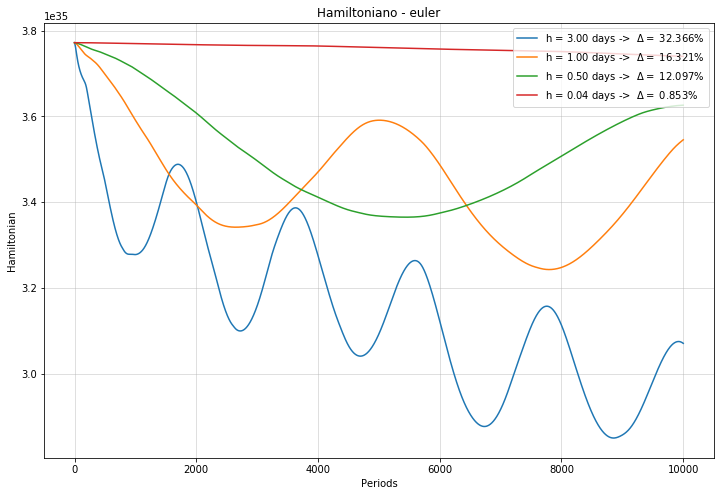
\includegraphics[width=50mm, height = 30mm]{resources/h_euler.png}
      \end{figure}

      \begin{figure}[h]
        \vspace{-0.5cm}
        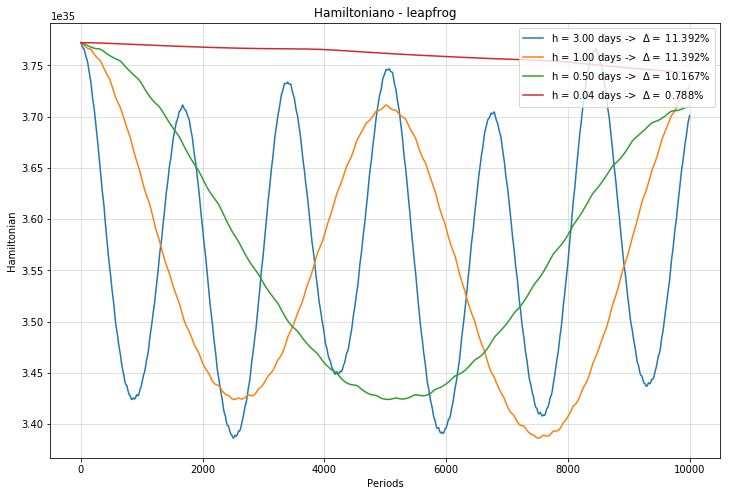
\includegraphics[width=50mm, height = 30mm]{resources/h_leap.png}
      \end{figure}

    \end{frame}

    \begin{frame}{Metódo de Euler}

      \begin{figure}[h]
        \vspace{-0.5cm}
        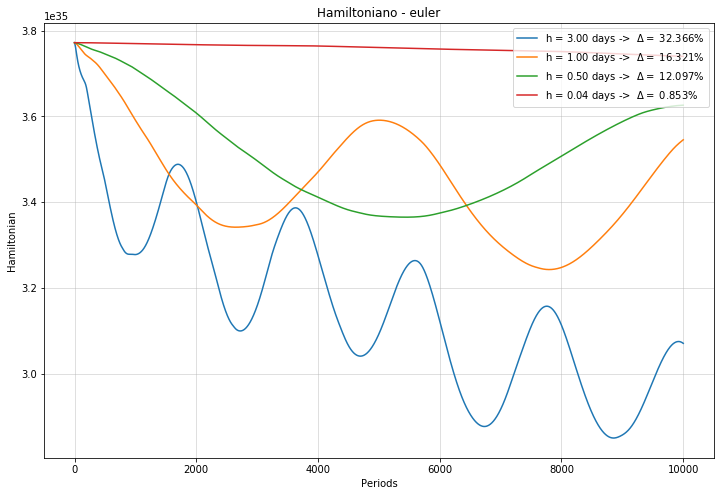
\includegraphics[width=100mm, height = 90mm]{resources/h_euler.png}
      \end{figure}

    \end{frame}

    \begin{frame}{Leapfrog}

      \begin{figure}[h]
        \vspace{-0.5cm}
        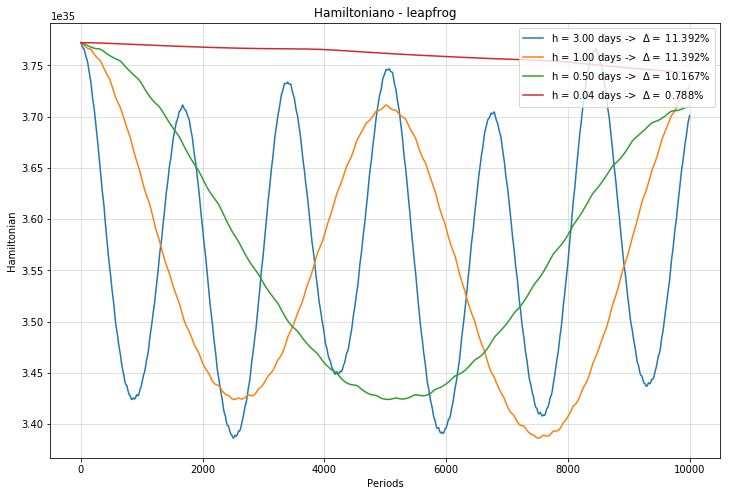
\includegraphics[width=100mm, height = 90mm]{resources/h_leap.png}
      \end{figure}

    \end{frame}

    \begin{frame}{Conservação do Momento Angular}

      \begin{figure}[h]
        \vspace{-0.5cm}
        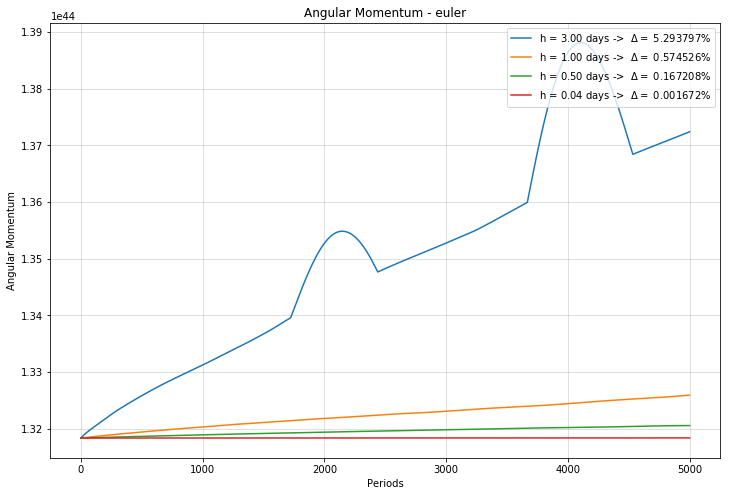
\includegraphics[width=50mm, height = 30mm]{resources/an_euler.png}
      \end{figure}

      \begin{figure}[h]
        \vspace{-0.5cm}
        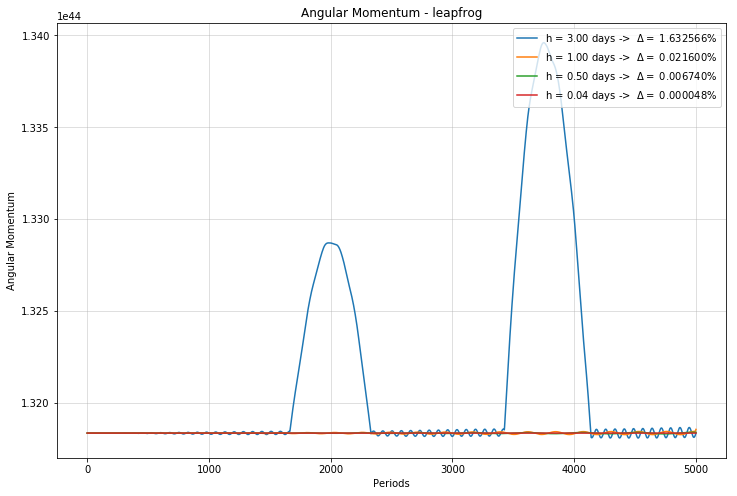
\includegraphics[width=50mm, height = 30mm]{resources/an_leap.png}
      \end{figure}

    \end{frame}

    \begin{frame}{Metódo de Euler}

      \begin{figure}[h]
        \vspace{-0.5cm}
        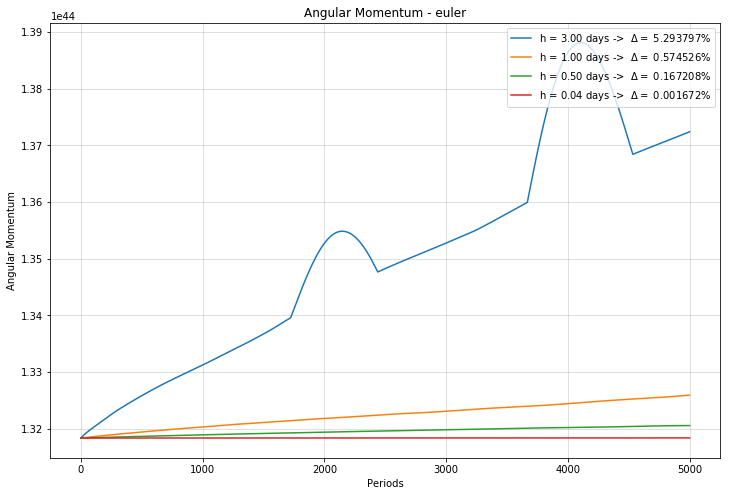
\includegraphics[width=100mm, height = 90mm]{resources/an_euler.png}
      \end{figure}

    \end{frame}

    \begin{frame}{Leapfrog}

      \begin{figure}[h]
        \vspace{-0.5cm}
        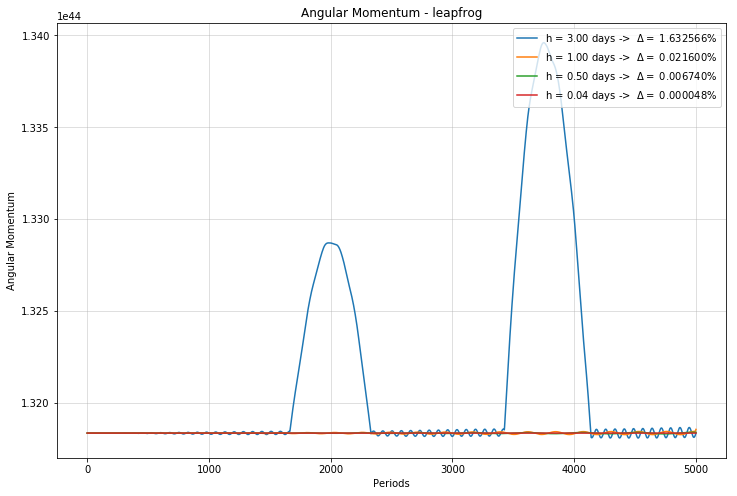
\includegraphics[width=100mm, height = 90mm]{resources/an_leap.png}
      \end{figure}

    \end{frame}

    %
    \begin{frame}{Metódo de Euler}

      \begin{figure}[h]
        \vspace{-0.5cm}
        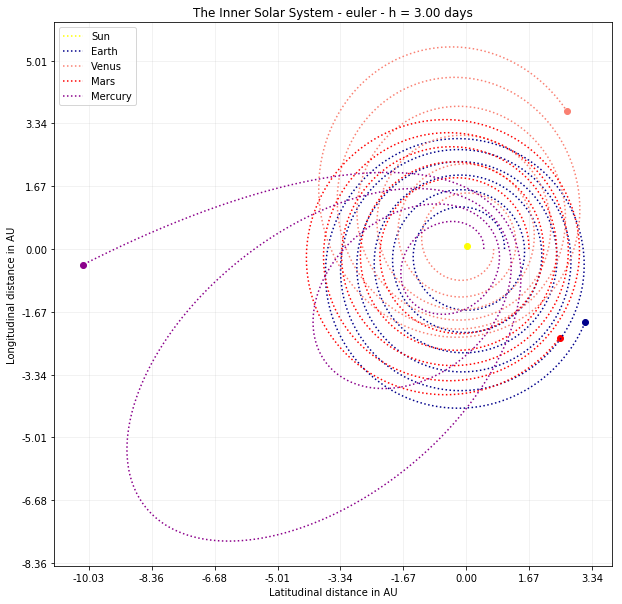
\includegraphics[width=100mm, height = 80mm]{resources/earth_wrong.png}
      \end{figure}

    \end{frame}

    \begin{frame}{Leapfrog}

      \begin{figure}[h]
        \vspace{-0.5cm}
        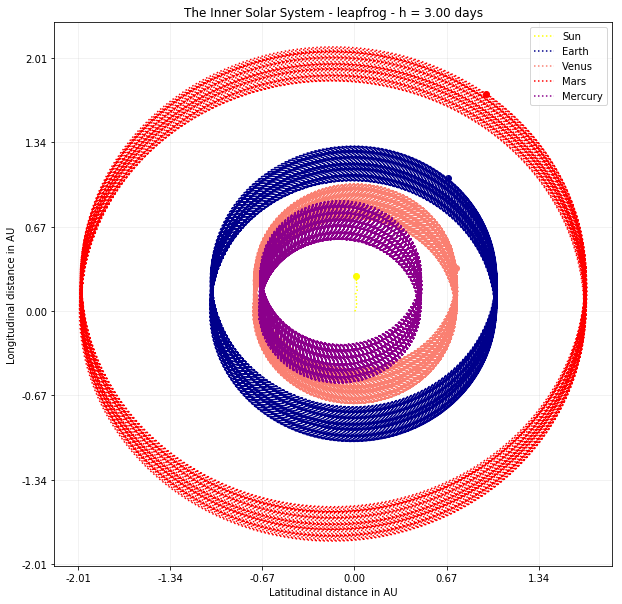
\includegraphics[width=100mm, height = 80mm]{resources/leap3.png}
      \end{figure}

    \end{frame}

    \begin{frame}{Euler-Cromer}

      \begin{figure}[h]
        \vspace{-0.5cm}
        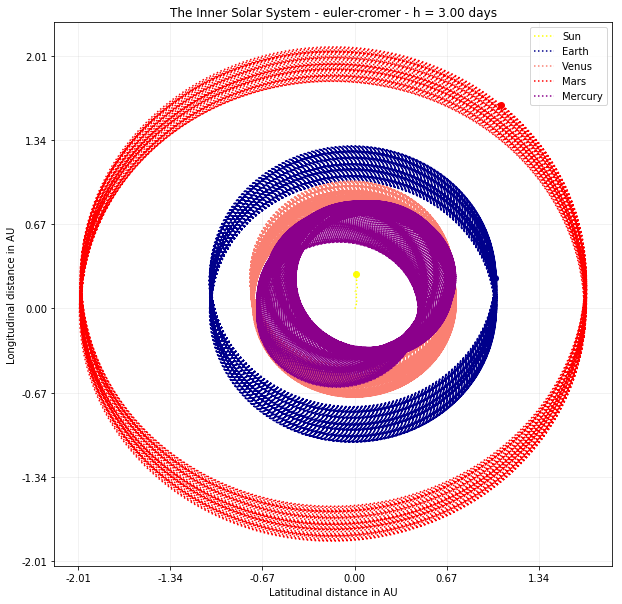
\includegraphics[width=100mm, height = 80mm]{resources/cromer3.png}
      \end{figure}

    \end{frame}

    \begin{frame}{Velocity Verlet}

      \begin{figure}[h]
        \vspace{-0.5cm}
        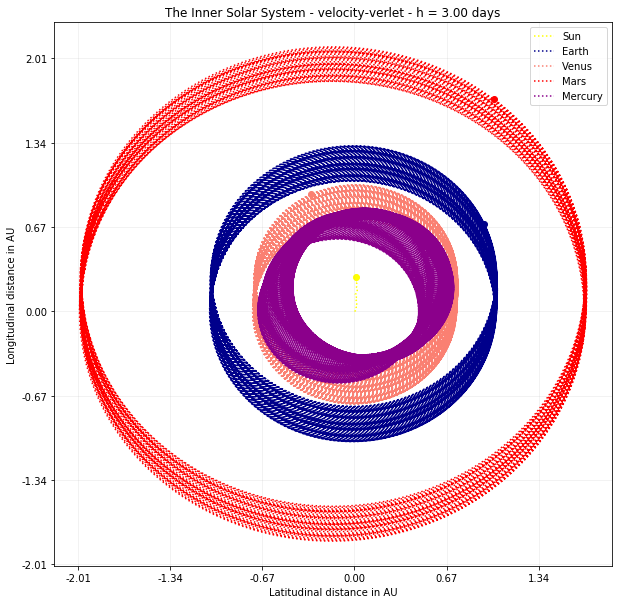
\includegraphics[width=100mm, height = 80mm]{resources/verlet3.png}
      \end{figure}

    \end{frame}

\begin{frame}
    \begin{table}[H]
    \centering
    \caption{Comparação da ecentricidade das órbitas}
    \label{tab:exTable1}
    \smallskip
    \begin{tabular}{|l|c|c|}
    \hline
    & Leapfrog Value & NASA Data\\[0.5ex]
    \hline
    &&\\[-2ex]
    Mercury & 0.196 & 0.206\\[0.5ex]
    \hline
    &&\\[-2ex]
    Venus & 0.018 & 0.007\\[0.5ex]
    \hline
    &&\\[-2ex]
    Earth & 0.0164 & 0.017\\[0.5ex]
    \hline
    &&\\[-2ex]
    Mars & 0.09 & 0.093\\[0.5ex]
    \hline
    &&\\[-2ex]
    Jupiter & 0.05 & 0.048\\[0.5ex]
    \hline
    \end{tabular}
    \end{table}
\end{frame}

\begin{frame}
  \begin{figure}[h]
    \vspace{-0.5cm}
    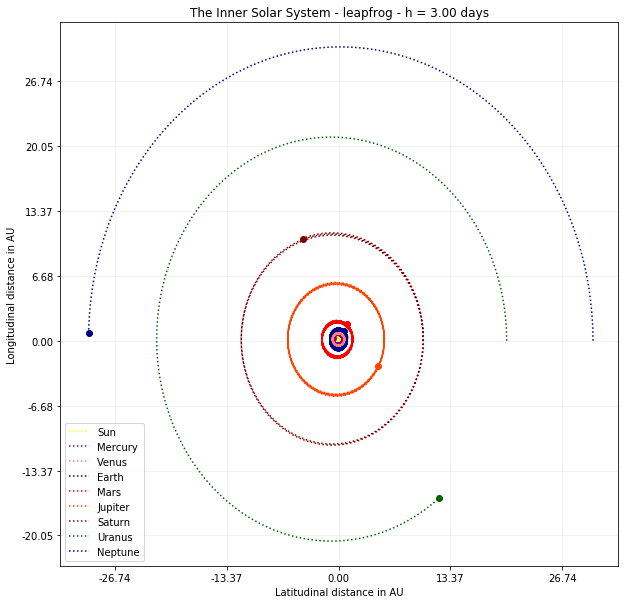
\includegraphics[width=110mm, height = 90mm]{resources/outer.png}
  \end{figure}
\end{frame}

    \begin{frame}{Muito Obrigado!}
      \framesubtitle{Carl Sagan}

      \begin{block}{}
        Diante da vastidão do \alert{tempo} e da imensidão do \alert{universo}, é um prazer para mim dividir um \alert{planeta} e uma \alert{época} com vocês.
      \end{block}
    \end{frame}
\end{document}
